\section*{Appendix}

\subsection{Compliance and reproducibility}

All submitted panels are produced by fixed automated pipelines without manual pixel editing or per-story prompt rewrites after viewing outputs.
General rules---subject-type normalization for humans, animals, and robots---apply uniformly and are not story-specific hard coding.
The LLM is used only for text-side structured planning; image synthesis runs locally on open checkpoints (SDXL-Turbo, IP-Adapter, StoryDiffusion, PixArt-$\alpha$, CLIP).
The system is not an agent that inspects images and autonomously revises prompts; generation, optional scoring, routing, and logging are predetermined stages.



\subsection{Anchor bank selection}

For each recurring subject, the anchor bank converts the structured character description into a visual reference prompt and generates several candidate identity anchors before story-level generation begins.  This keeps the identity reference independent from any single story panel: the chosen anchor is later reused by IP-Adapter whenever the routing policy selects identity conditioning for that character.

The example is taken from \texttt{04.txt}.  The manual character payload specifies a young child with short brown hair, a blue T-shirt, and jeans.  The anchor bank turns this metadata into the following half-body reference prompt:
\begin{quote}
\footnotesize
``a single young child with short brown hair, wearing a blue t-shirt and jeans, full-body identity reference, standing alone, centered, simple plain background, one child only, clean cartoon illustration style.''
\end{quote}

The pipeline generated three half-body candidates using consecutive seeds 900001--900003.  Each candidate was checked for basic validity and then scored with the CLIP text-image selector configured as \texttt{clip\_text\_alignment}.  The selector score is computed as \texttt{clip\_alignment} plus \texttt{quality\_score}.  The quality score is a lightweight image-validity term: 0.5 if the file exists and 0.5 if the image can be opened.  In this run all three images were valid, so the CLIP text alignment term determined the final ranking.  The selector log reports no CLIP errors for any candidate.

\begin{table}[!h]
  \centering
  \scriptsize
  \setlength{\tabcolsep}{3pt}
  \caption{Anchor selector scores for the Milo half-body candidates.}
  \label{tab:milo_anchor_scores}
  \begin{tabular}{ccccc}
    \toprule
    Cand. & Seed & CLIP align. & Quality & Selector \\
    \midrule
    0 & 900001 & 0.398654 & 1.000000 & 1.398654 \\
    1 & 900002 & 0.369347 & 1.000000 & 1.369347 \\
    2 & 900003 & 0.370939 & 1.000000 & 1.370939 \\
    \bottomrule
  \end{tabular}
\end{table}

Figure~\ref{fig:anchor_milo} shows the three candidates and the canonical reference copied into the anchor bank.  Candidate 0 has the highest selector score in Table~\ref{tab:milo_anchor_scores}, so it becomes \texttt{canonical\_half\_body.png}.  This selected canonical anchor is then passed to IP-Adapter as the visual identity condition for subsequent single-subject panel generation.

\begin{figure}[!h]
  \centering
  \begin{subfigure}{0.24\columnwidth}
    
\includegraphics[width=\linewidth]{figs/anchor_milo_candidate_0.png}
    \caption{Cand.~0}
  \end{subfigure}\hfill
  \begin{subfigure}{0.24\columnwidth}
    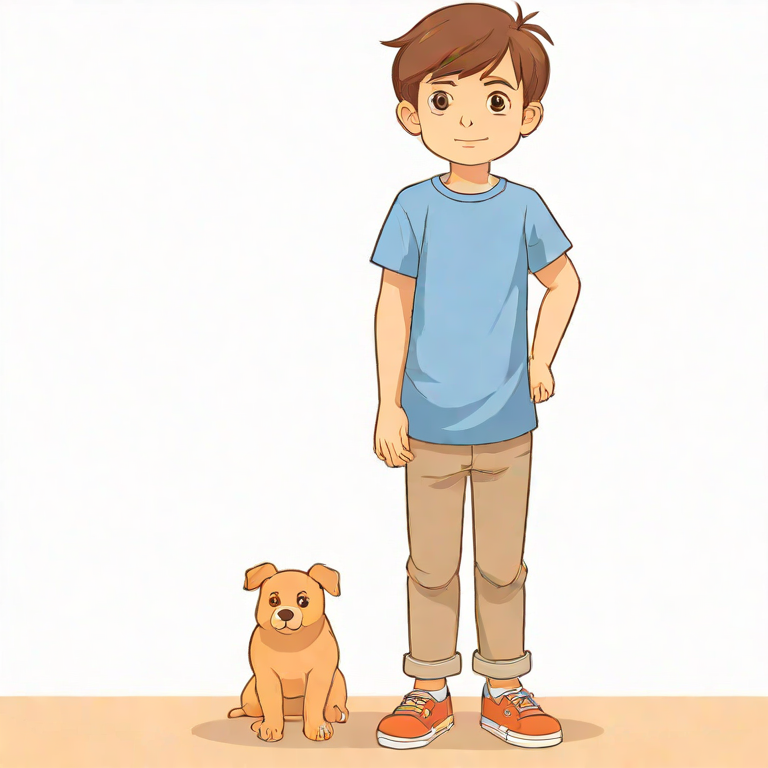
\includegraphics[width=\linewidth]{figs/anchor_milo_candidate_1.png}
    \caption{Cand.~1}
  \end{subfigure}\hfill
  \begin{subfigure}{0.24\columnwidth}
    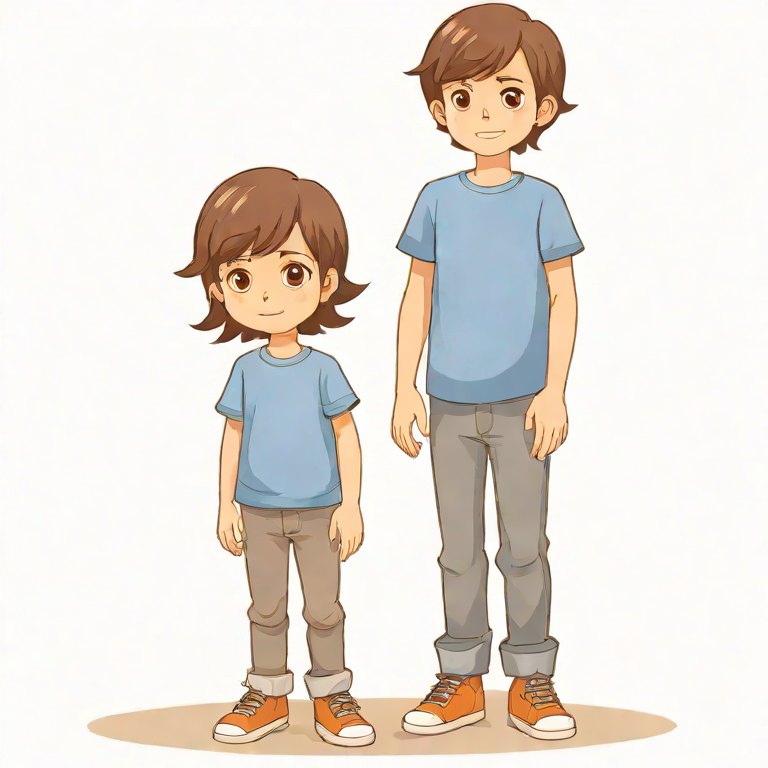
\includegraphics[width=\linewidth]{figs/anchor_milo_candidate_2.png}
    \caption{Cand.~2}
  \end{subfigure}\hfill
  \begin{subfigure}{0.24\columnwidth}
    
\includegraphics[width=\linewidth]{figs/anchor_milo_canonical_half_body.png}
    \caption{Canonical}
  \end{subfigure}
  \caption{Milo anchor bank candidates and selected canonical half-body identity anchor.}
  \label{fig:anchor_milo}
\end{figure}

\subsection{IP-Adapter on versus off}

\begin{figure}[!h]
  \centering
  \begin{subfigure}{0.48\columnwidth}
    \fbox{\parbox[c][0.75in][c]{0.95\linewidth}{\centering\scriptsize without IP-Adapter\\PLACEHOLDER}}
    \caption{Off}
  \end{subfigure}
  \hfill
  \begin{subfigure}{0.48\columnwidth}
    \fbox{\parbox[c][0.75in][c]{0.95\linewidth}{\centering\scriptsize with IP-Adapter\\PLACEHOLDER}}
    \caption{On}
  \end{subfigure}
  \caption{Single-character story: identity drift without visual conditioning (left) vs.\ anchor-conditioned generation (right).}
  % USER: two-panel comparison from ablation run
\end{figure}

\subsection{Native identity reference failure}

\begin{figure}[!h]
  \centering
  \fbox{\parbox[c][0.85in][c]{0.95\columnwidth}{\centering\scriptsize Identity ref frame\\(character sheet / multi-view)\\PLACEHOLDER}}
  \caption{StoryDiffusion identity reference degenerating into a character sheet, weakening the identity bank.}
  \label{fig:identity_sheet}
  % USER: fig_native_identity_ref_sheet.pdf
\end{figure}

\subsection{DiT supplementary cases}

\begin{figure}[!h]
  \centering
  \begin{subfigure}{0.48\columnwidth}
    \includegraphics[width=\linewidth]{figs/dit_best.png}
    \caption{Best: PixArt+LoRA, Story-01}
  \end{subfigure}
  \hfill
  \begin{subfigure}{0.48\columnwidth}
    \includegraphics[width=\linewidth]{figs/dit_failure.png}
    \caption{Failure: identity drift}
  \end{subfigure}
  \caption{DiT best vs.\ failure. (a) Scene-level LoRA with simple prompt on Story-01: three panels show the same character. (b) Story-joint blending run: cross-scene attention dilutes LoRA identity, producing noticeably different faces across panels.}
  \label{fig:dit_supp}
  % USER: figs/dit_best.png  = 1 panel from dit_lora_smoke_full_*/generation/scenes/scene_001/selected.png
  %       figs/dit_failure.png = 1 panel from a story-joint blending run (different person per panel)
\end{figure}

\subsection{DiT training data samples}

\begin{figure}[!h]
  \centering
  \begin{subfigure}{0.32\columnwidth}
    \includegraphics[width=\linewidth]{figs/dit_train_canonical.png}
    \caption{Canonical}
  \end{subfigure}
  \hfill
  \begin{subfigure}{0.32\columnwidth}
    \includegraphics[width=\linewidth]{figs/dit_train_aug1.png}
    \caption{Flip augment}
  \end{subfigure}
  \hfill
  \begin{subfigure}{0.32\columnwidth}
    \includegraphics[width=\linewidth]{figs/dit_train_aug2.png}
    \caption{Crop augment}
  \end{subfigure}
  \caption{DiT DreamBooth LoRA training data: canonical anchor portrait (left) and two augmentation variants (center, right). All 10--16 training images derive from the same single generated portrait via flips, crops, and brightness adjustments.}
  \label{fig:dit_train}
  % USER: figs/dit_train_canonical.png = Lily_canonical.png from training_images/
  %       figs/dit_train_aug1.png = any Lily_diverse_*.png from training_images/
  %       figs/dit_train_aug2.png = another Lily_diverse_*.png from training_images/
\end{figure}


